\documentclass[12pt,xcolor=dvipsnames]{beamer}
\usecolortheme[named=Maroon]{structure}
\usetheme{Luebeck}
\usepackage[utf8]{inputenc}
\usepackage{amsmath}
\usepackage{amsfonts}
\usepackage{amssymb}
\usepackage{graphicx}
\DeclareMathOperator\erfc{erfc}
\graphicspath{{../plots/}}
\author{Jonathan Morrell}
\title{$^{nat}$La(p,x) XS Review}
%\setbeamercovered{transparent} 
%\setbeamertemplate{navigation symbols}{} 
%\logo{} 
%\institute{} 
%\date{} 
%\subject{} 
\begin{document}

\begin{frame}
\titlepage
\end{frame}

%\begin{frame}
%\tableofcontents
%\end{frame}

\begin{frame}
\frametitle{Methodology}
\begin{itemize}
\item Fitting calibration peaks
\item Detector calibration
\item Fitting monitor and target peaks
\item Determining end-of-beam activities ($A_0$)
\item Determining beam current and energies
\item Generate cross-sections
\item Compare results to EXFOR, TALYS and EMPIRE
\end{itemize}
\end{frame}

\begin{frame}
\frametitle{Cross-section Equations}
\begin{columns}[c]
\column{2.5in}
$A_0 = \frac{\lambda N_c}{(1-e^{-\lambda t_m})e^{-\lambda t_c}I_{\gamma}\epsilon}$
\\
$A_0 = \sigma I_p \rho \Delta r (1-e^{-\lambda t_i})$
\column{1.5in}
$A_0$: End-of-beam activity\\
$t_m$: Measurement time\\
$t_c$: Cooling time\\
$t_i$: Irradiation time\\
$I_p$: Beam current\\
$\rho \Delta r$: Areal density\\
\end{columns}
\end{frame}

\begin{frame}
\frametitle{Peak Fitting}
Fit to a skewed Gaussian
\begin{align*}
F_{peak}(i) &= m\cdot i + b + A\cdot [\exp (-\frac{(i-\mu)^2}{2\sigma^2}) \\
& + R\cdot \exp (\frac{i-\mu}{\alpha \sigma}) \erfc (\frac{i-\mu}{\sqrt{2}\sigma}+\frac{1}{\sqrt{2}\alpha})]
\label{eq:peak}
\end{align*}
\centering
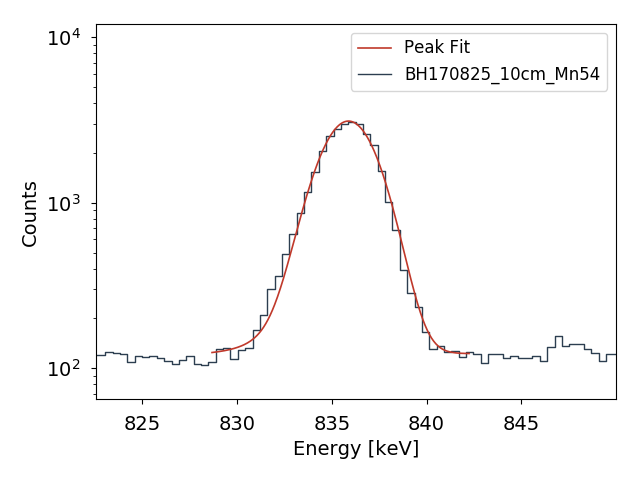
\includegraphics[width=2.0in]{Mn_Peak.png}
\end{frame}

\begin{frame}
\frametitle{Other Peak Examples}
\centering
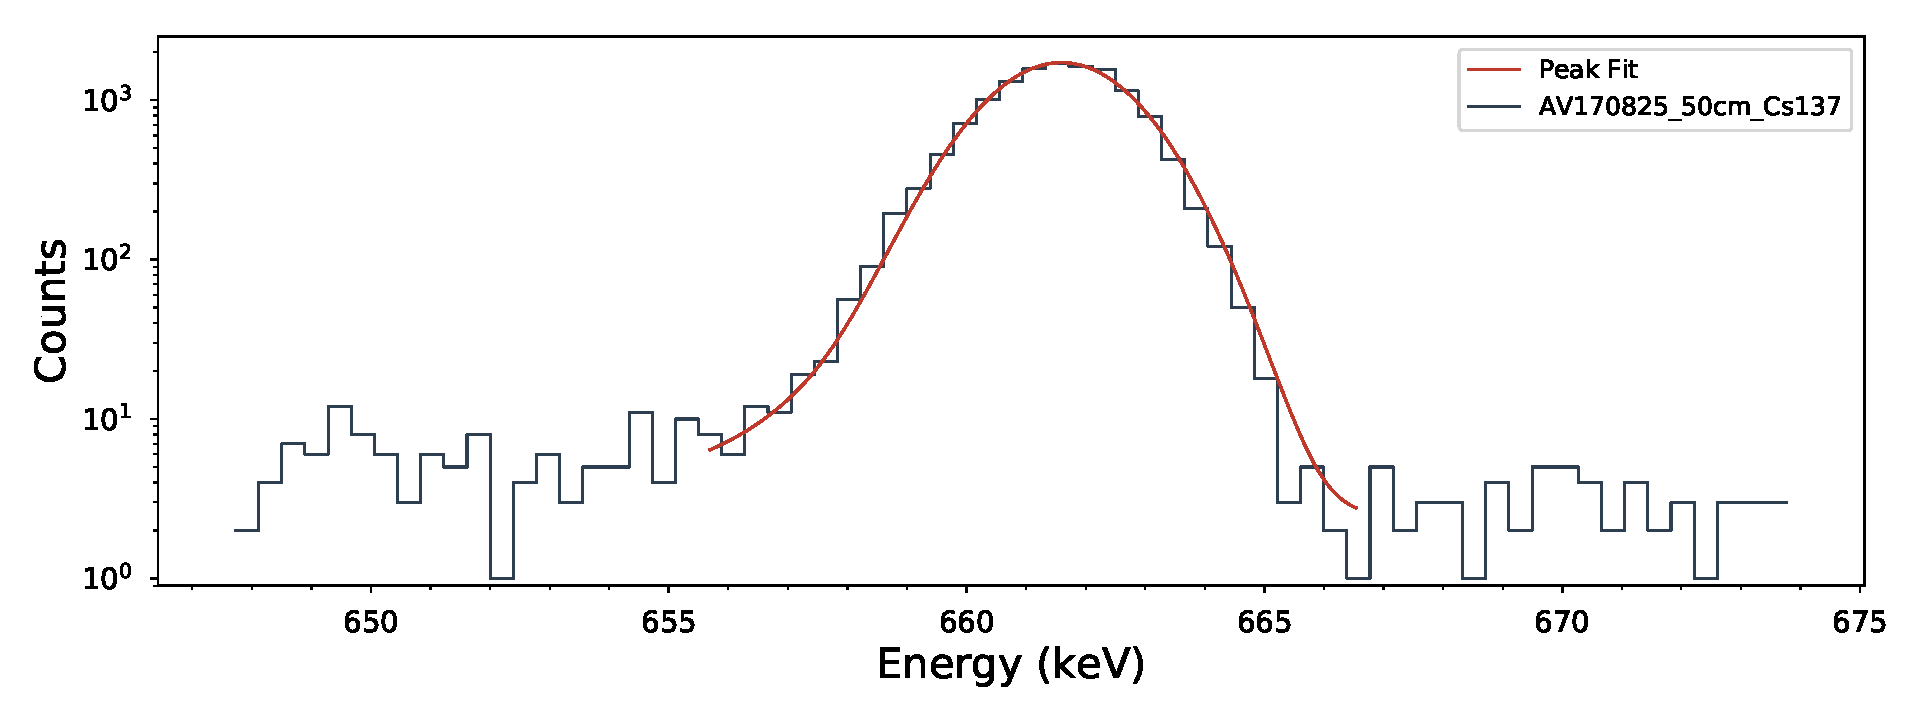
\includegraphics[width=4.0in]{peak_fits/AV170825_50cm_Cs137_fits}

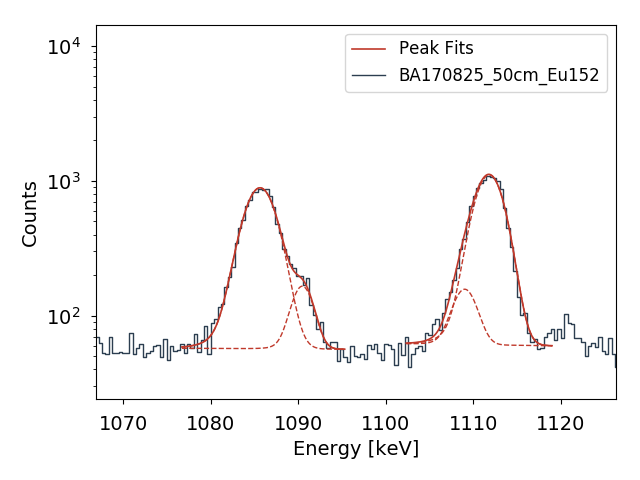
\includegraphics[width=2.0in]{Eu_Peaks.png}

\end{frame}

\begin{frame}
\frametitle{Calibration}
\begin{columns}[c]
\column{2.5in}
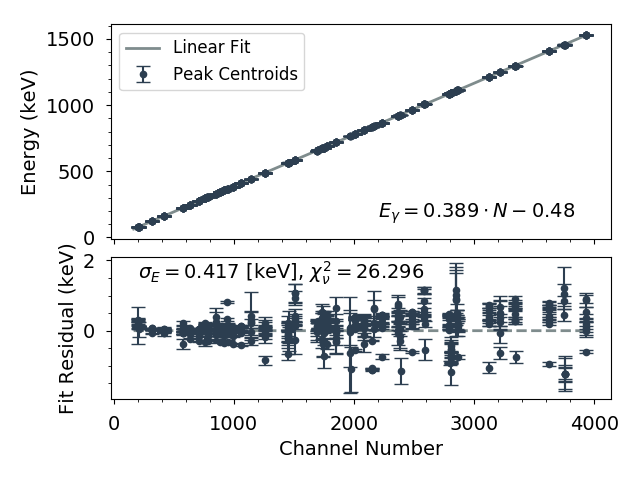
\includegraphics[width=2.5in]{calibration/energy_calibration}
\column{2.5in}
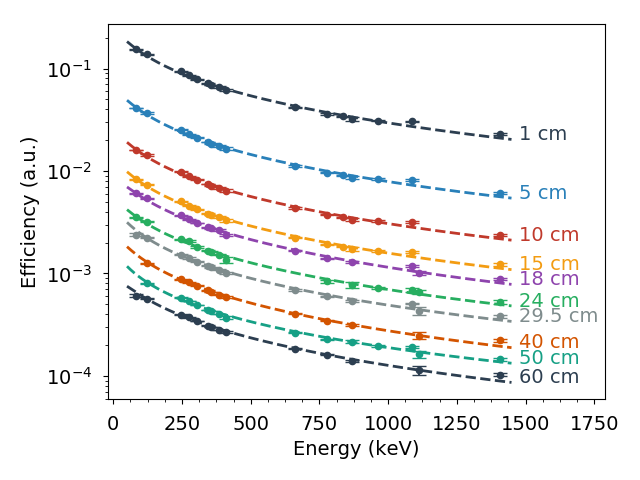
\includegraphics[width=2.5in]{calibration/efficiency_calibration}
\end{columns}
$E = m\cdot i+b$
\ \ \\
$\epsilon (E) = exp[a\cdot ln(E)^2+b\cdot ln(E)+c]$

\end{frame}

\begin{frame}
\frametitle{Fitting Monitor Peaks}
\centering
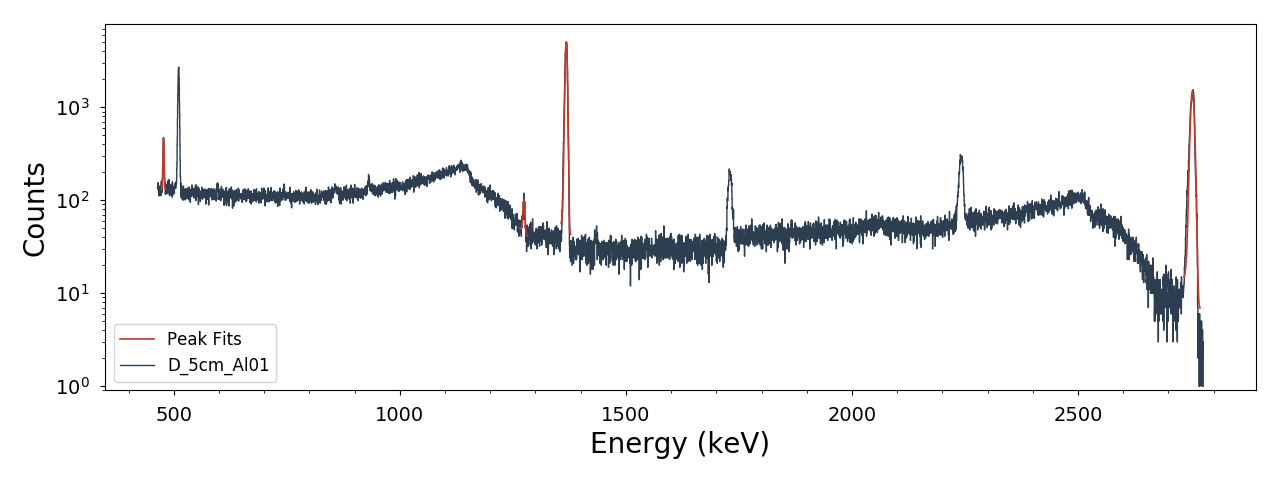
\includegraphics[width=4.0in]{peak_fits/D_5cm_Al01_fits}

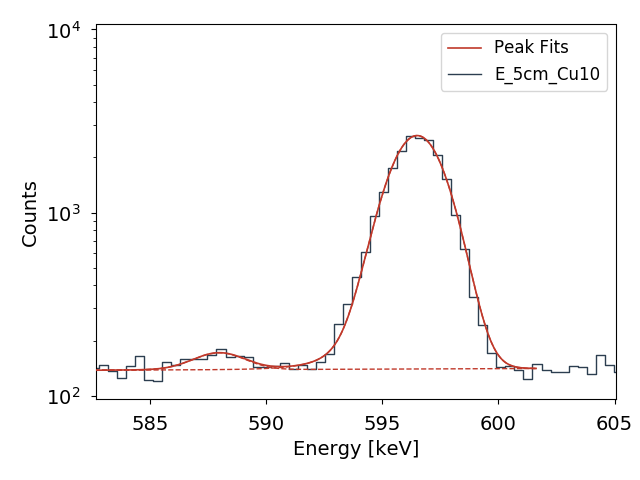
\includegraphics[width=2.0in]{62ZN_Peak.png}

\end{frame}

\begin{frame}
\frametitle{End-of-Beam Activities}
\begin{columns}[c]
\column{2.5in}
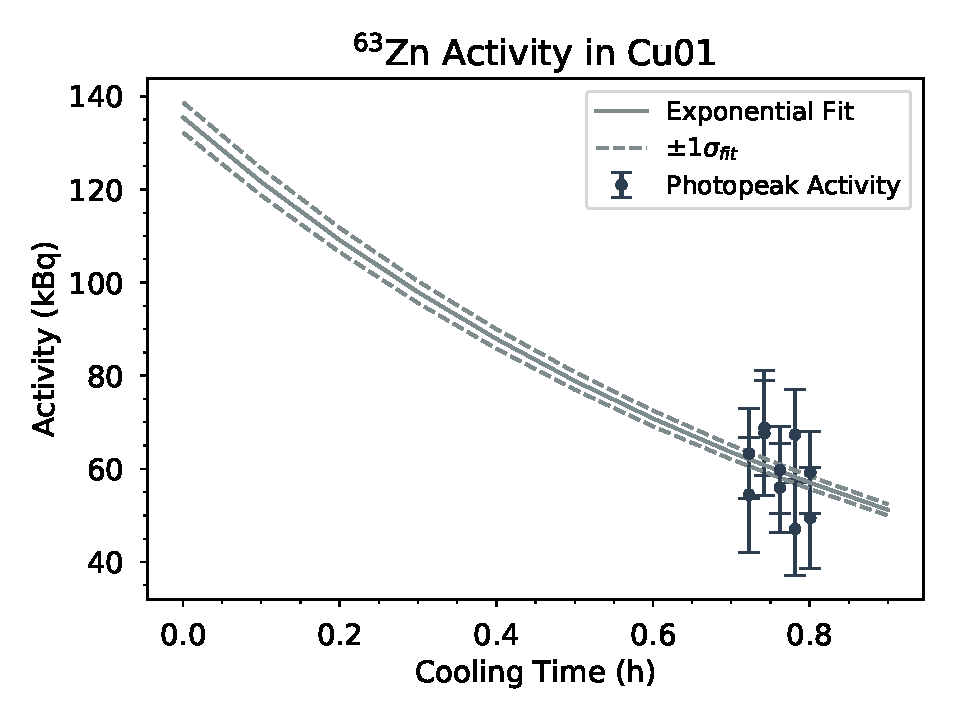
\includegraphics[width=2.5in]{decay_curves/Cu01_63ZN}
\column{2.5in}
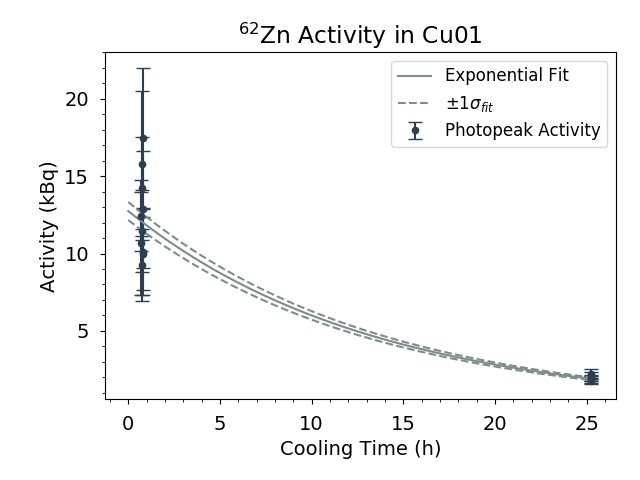
\includegraphics[width=2.5in]{decay_curves/Cu01_62ZN}
\end{columns}
\end{frame}

\begin{frame}
\frametitle{MCNP - Anderson Ziegler Comparison}
\begin{columns}[c]
\column{2.5in}
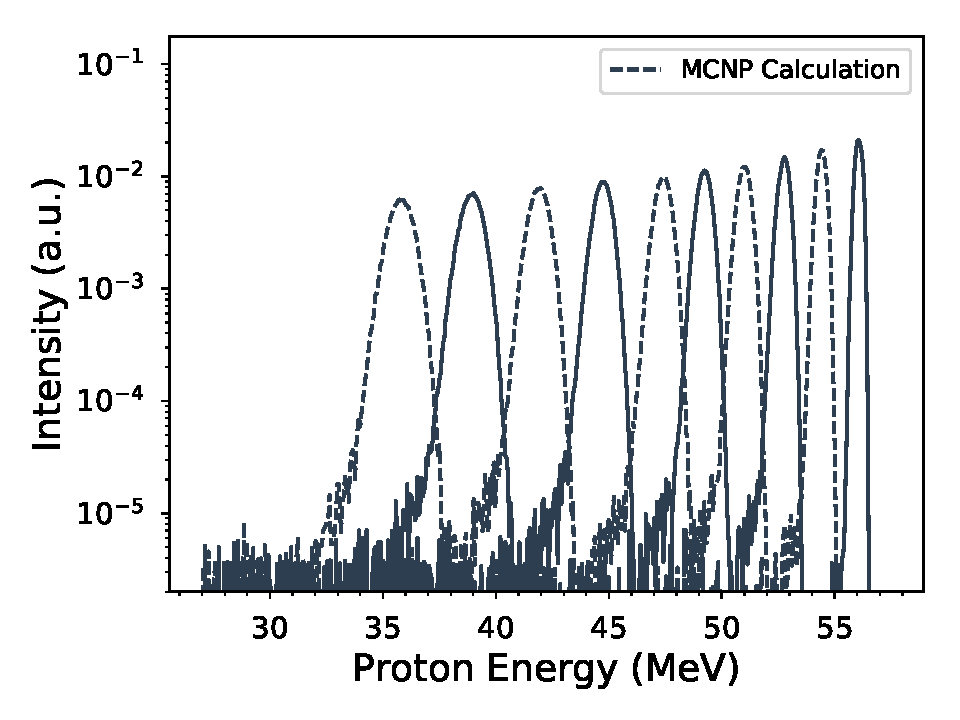
\includegraphics[width=2.5in]{monitors/La_mcnp_spectrum}
\column{2.5in}
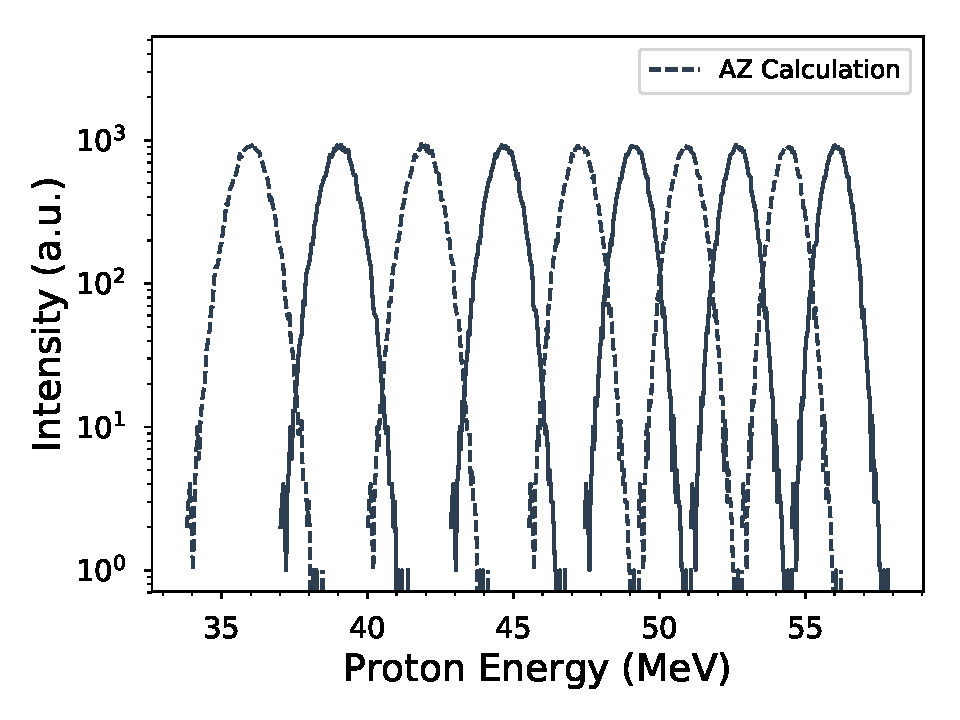
\includegraphics[width=2.5in]{monitors/La_az_spectrum}
\end{columns}
\end{frame}

\begin{frame}
\frametitle{Aluminum Monitor Corrections}
\begin{columns}[c]
\column{2.5in}
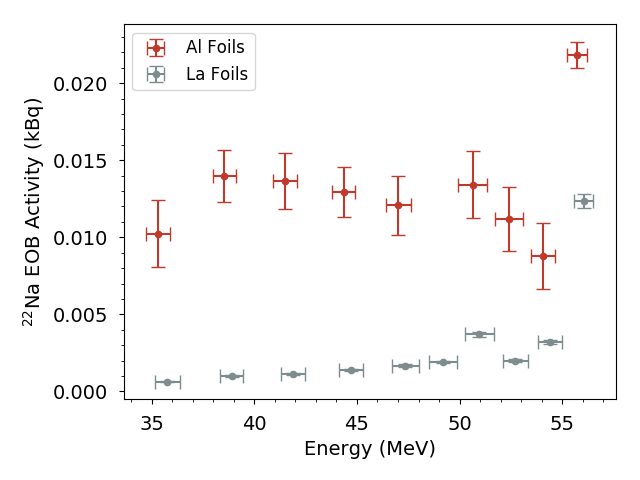
\includegraphics[width=2.5in]{monitors/22NA_Al_Correction}
\column{2.5in}
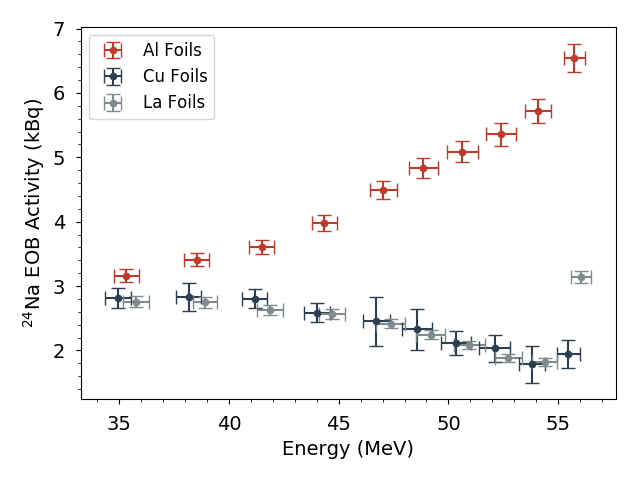
\includegraphics[width=2.5in]{monitors/24NA_Al_Correction}
\end{columns}
\end{frame}


\begin{frame}
\frametitle{Determining Beam Current}
\begin{columns}[c]
\column{1.5in}
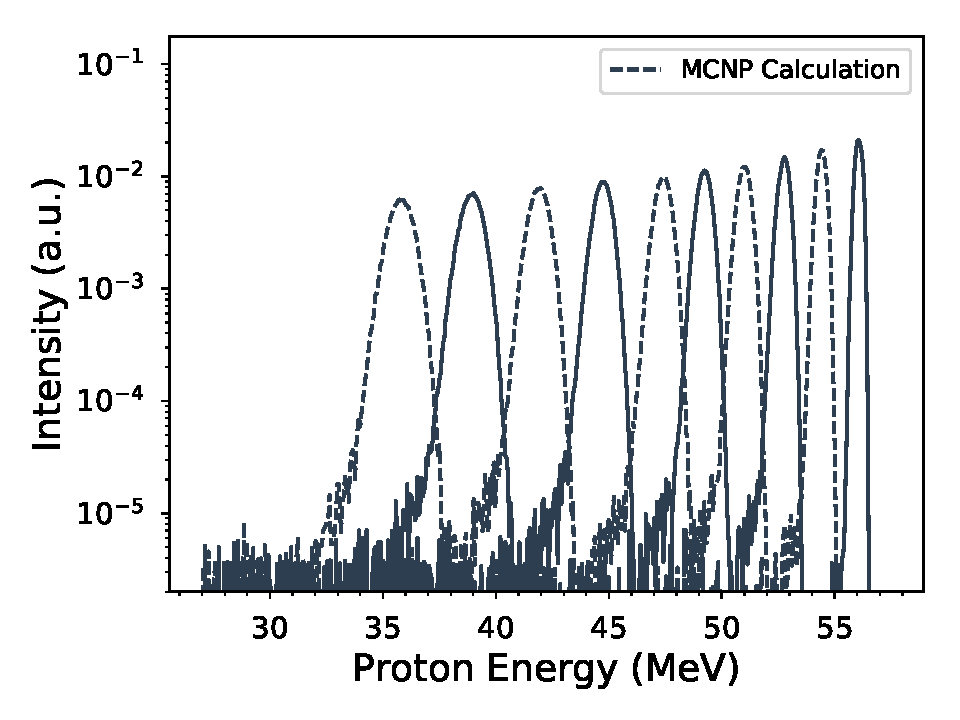
\includegraphics[width=1.5in]{monitors/La_mcnp_spectrum}
\\
Optimum $\Delta \rho$ determined by $\chi^2$ minimization using MCNP
\column{2.5in}
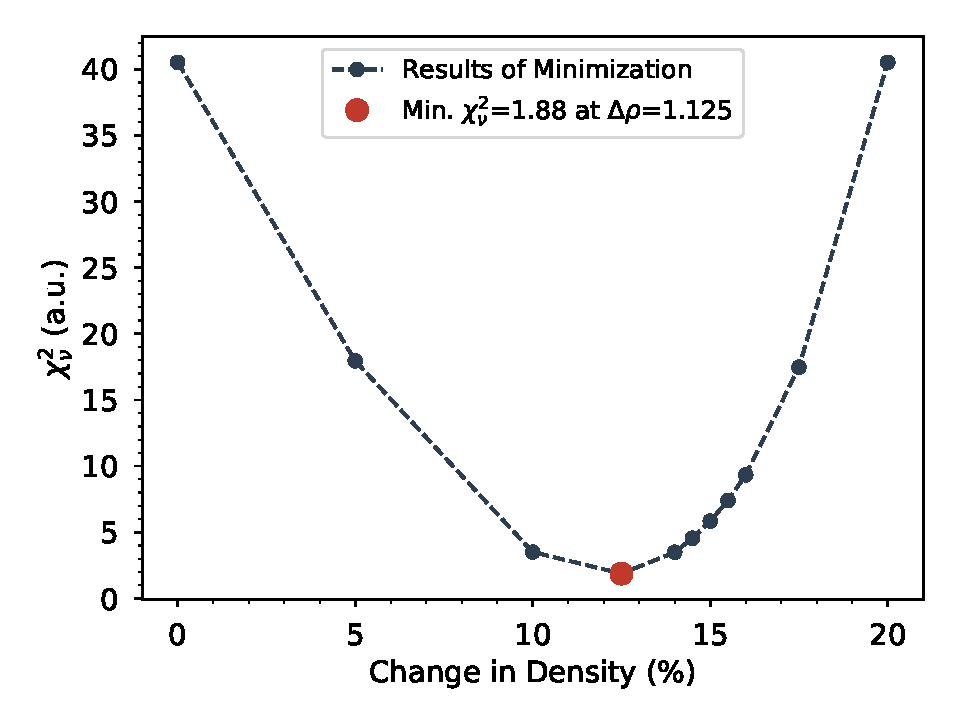
\includegraphics[width=2.5in]{monitors/minimize_mcnp}
\end{columns}
\end{frame}

\begin{frame}
\frametitle{Optimized Beam Current}
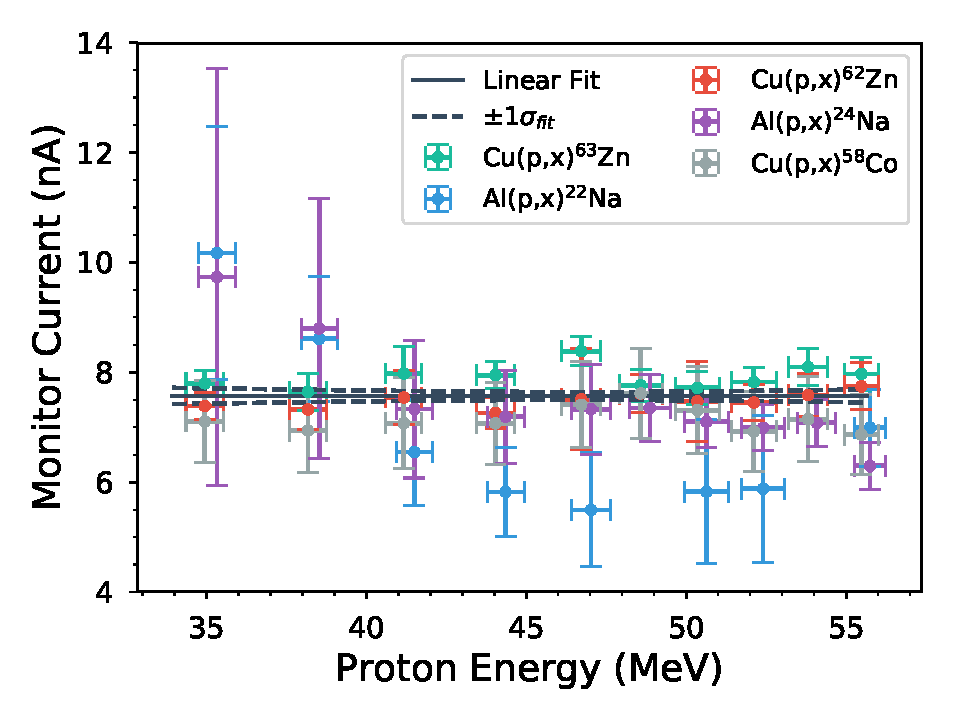
\includegraphics[width=3.5in]{monitors/current_norm_mcnp}
\\
Optimum value of $\Delta \rho$: 1.15
\end{frame}

\begin{frame}
\frametitle{Monitor Cross-Sections}
\begin{columns}[c]
\column{2.5in}
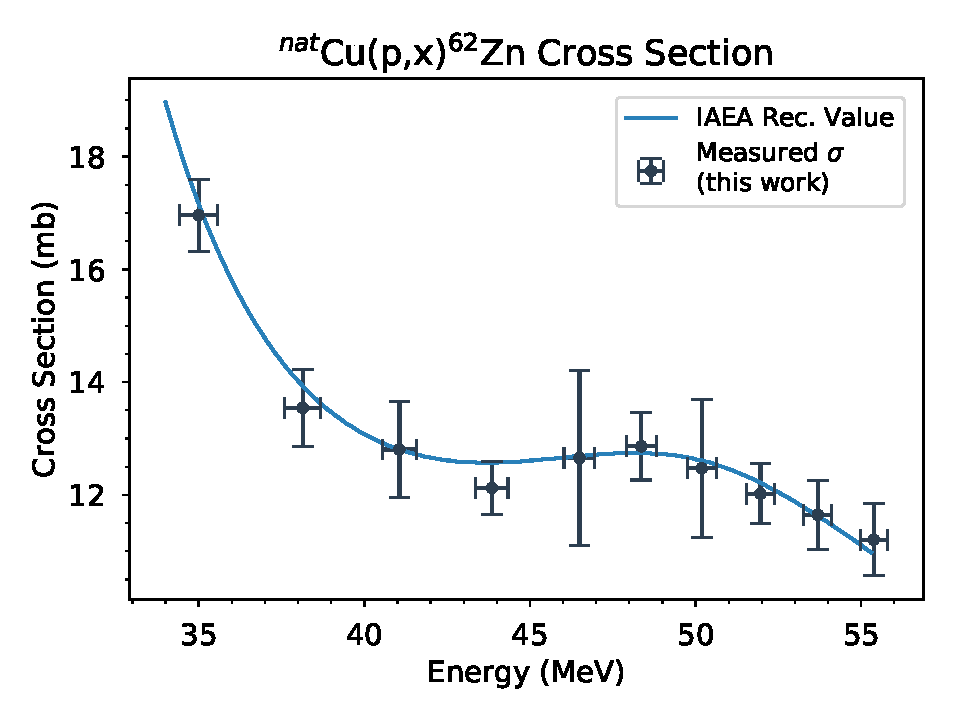
\includegraphics[width=2.5in]{cross_sections/62ZN}
\\
\centering
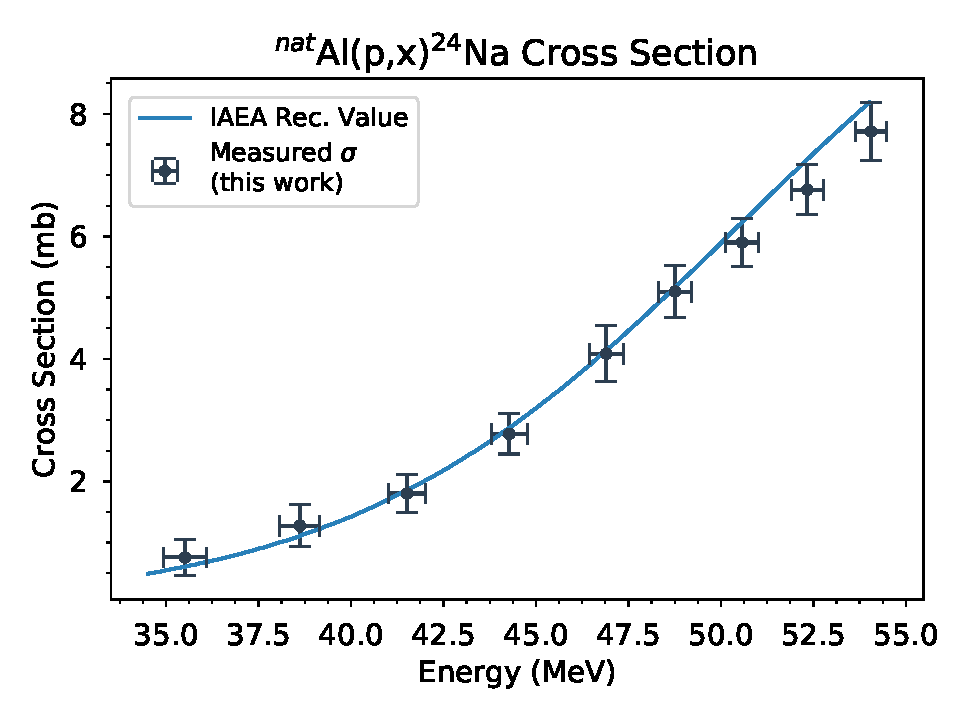
\includegraphics[width=2.0in]{cross_sections/24NA}
\\
\column{2.5in}
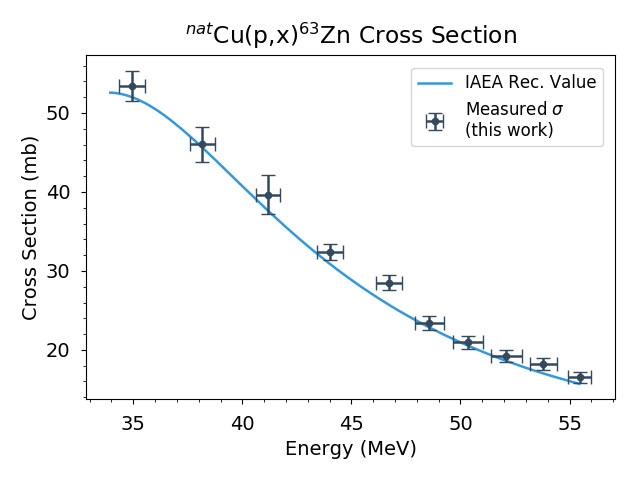
\includegraphics[width=2.5in]{cross_sections/63ZN}
\\
\centering
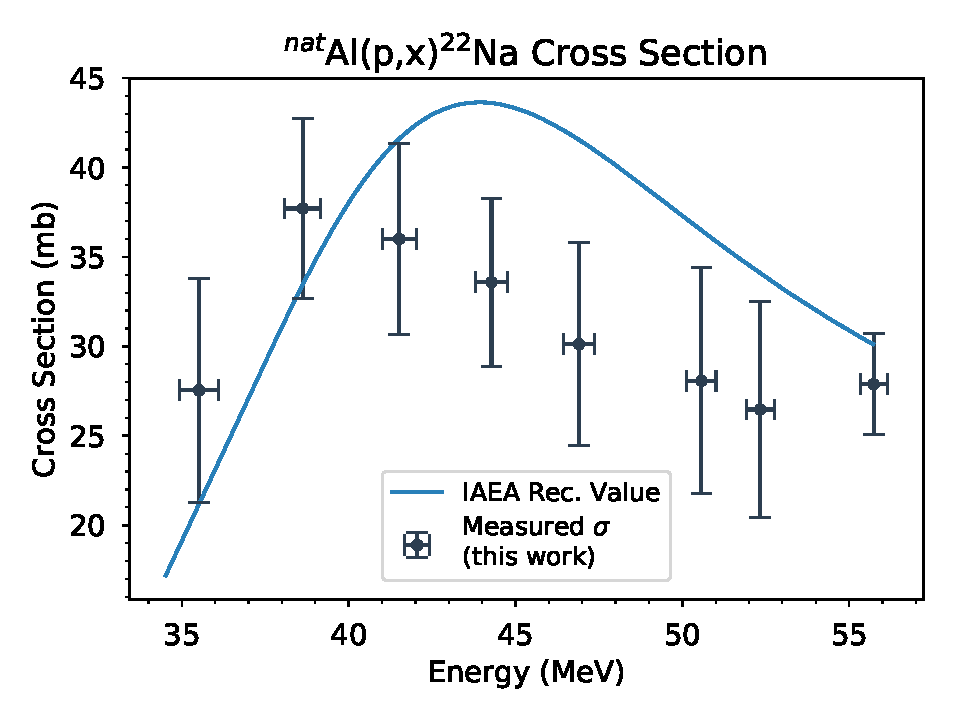
\includegraphics[width=2.0in]{cross_sections/22NA}
\\
\end{columns}
\end{frame}

\begin{frame}
\frametitle{Comparison to EXFOR Data}
\begin{columns}[c]
\column{2.5in}
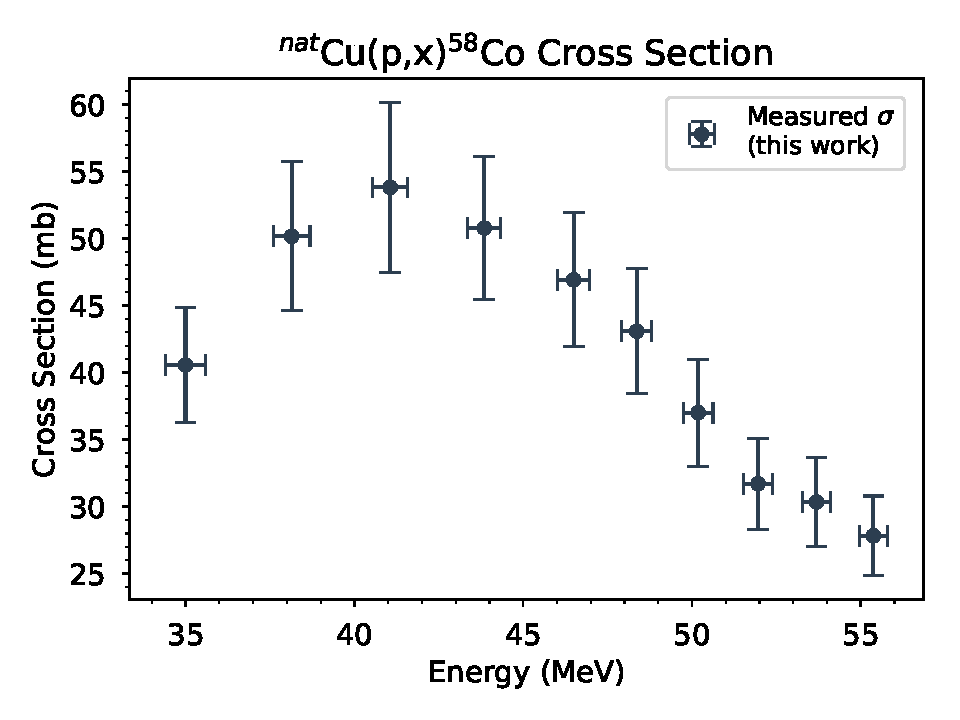
\includegraphics[width=2.5in]{cross_sections/58CO_only}
\\
\column{2.5in}
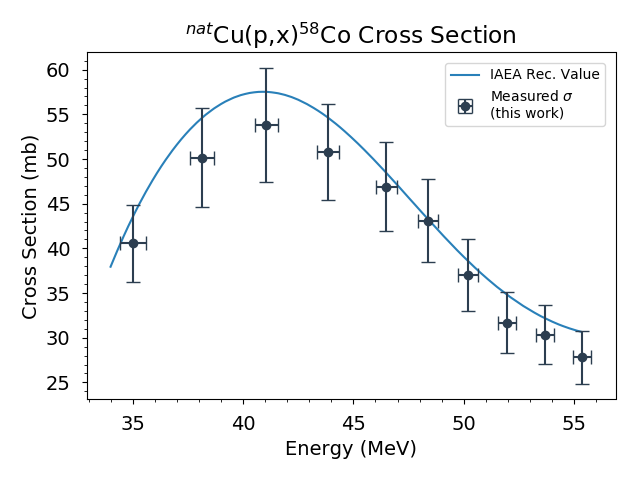
\includegraphics[width=2.5in]{cross_sections/58CO}
\\
\end{columns}
\end{frame}

\begin{frame}
\frametitle{Comparison to EXFOR Data}
\begin{columns}[c]
\column{2.5in}
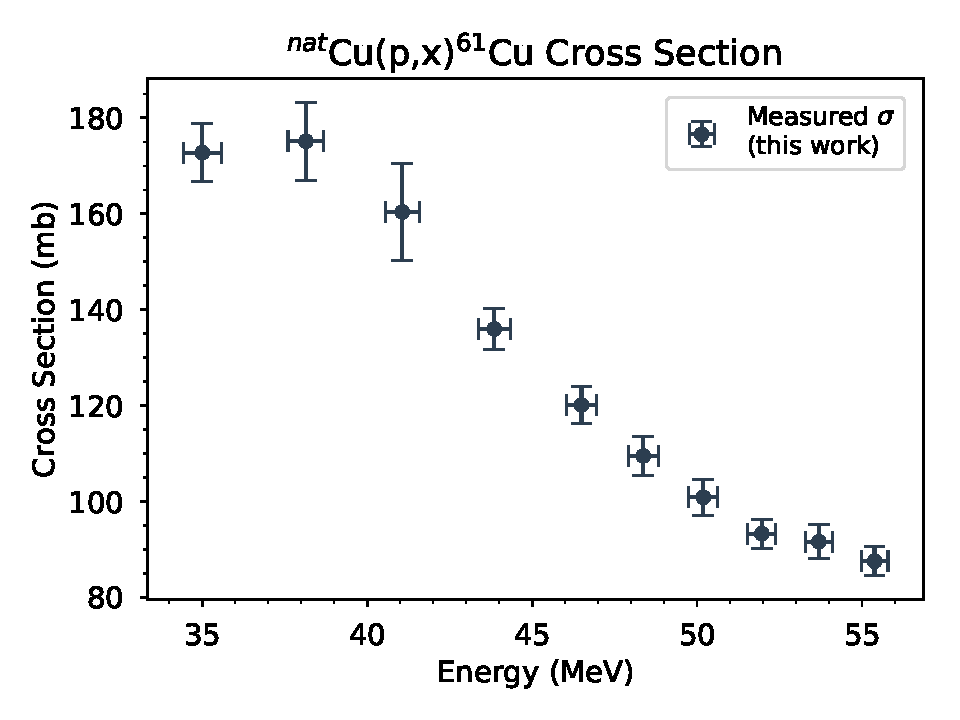
\includegraphics[width=2.5in]{cross_sections/61CU_only}
\\
\column{2.5in}
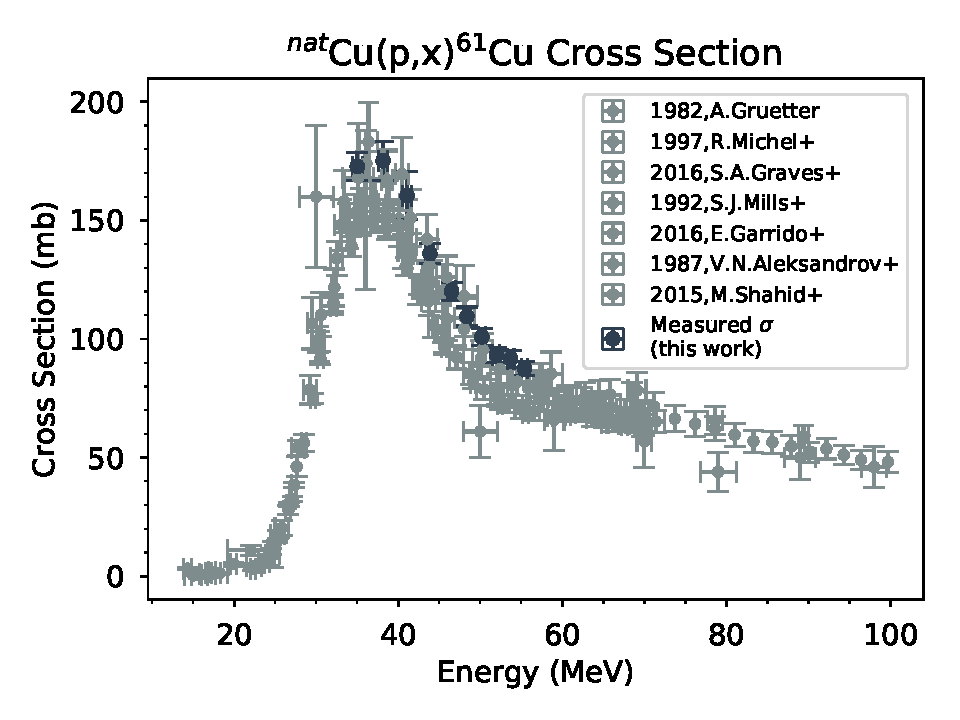
\includegraphics[width=2.5in]{cross_sections/61CU}
\\
\end{columns}
\end{frame}

\begin{frame}
\frametitle{Peak Fitting of Lanthanum Data}
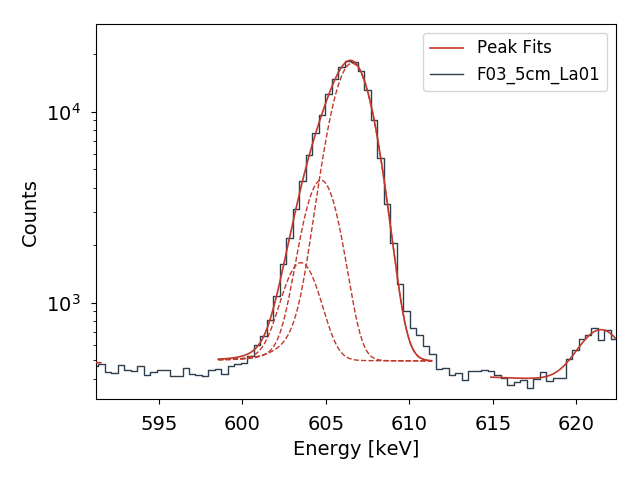
\includegraphics[width=4.0in]{early_604.png}
\end{frame}

\begin{frame}
\frametitle{Peak Fitting of Lanthanum Data}
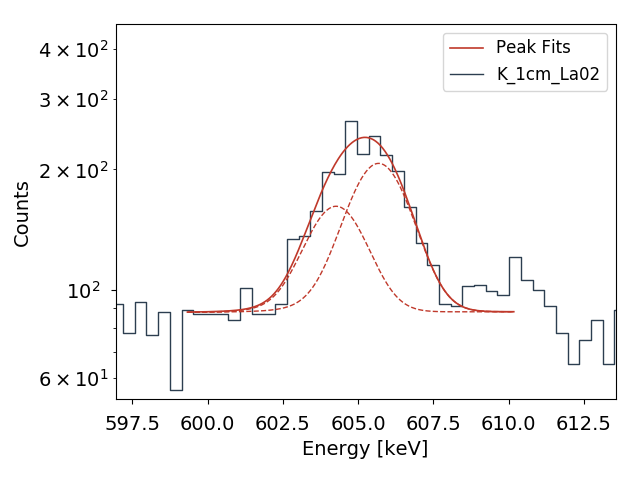
\includegraphics[width=4.0in]{intermediate_604.png}
\end{frame}

\begin{frame}
\frametitle{Peak Fitting of Lanthanum Data}
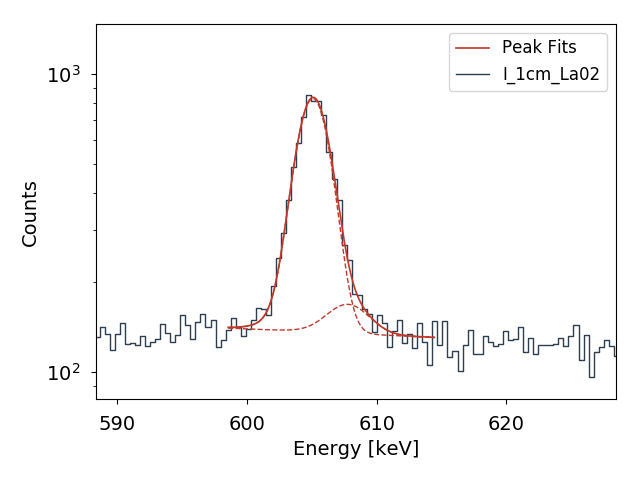
\includegraphics[width=4.0in]{late_604.png}
\end{frame}

\begin{frame}
\frametitle{Calculate $^{134}Ce$ $A_0$ from $^{134}La$ $A(t_c)$}
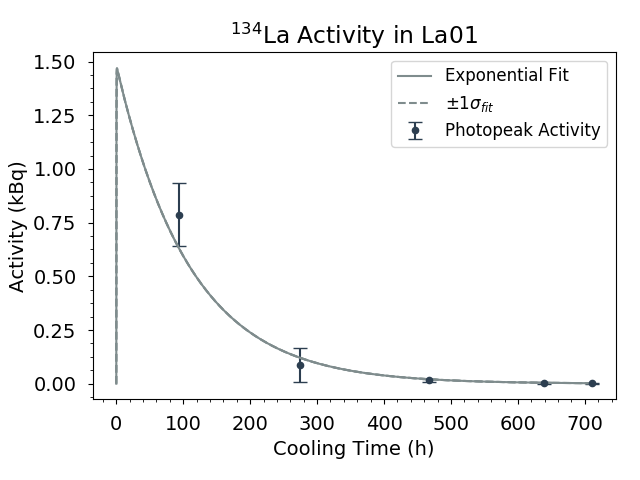
\includegraphics[width=4.0in]{decay_curves/La01_134LA}
\end{frame}

\begin{frame}
\frametitle{Comparison to previous analysis}
\begin{columns}[c]
\column{2.5in}
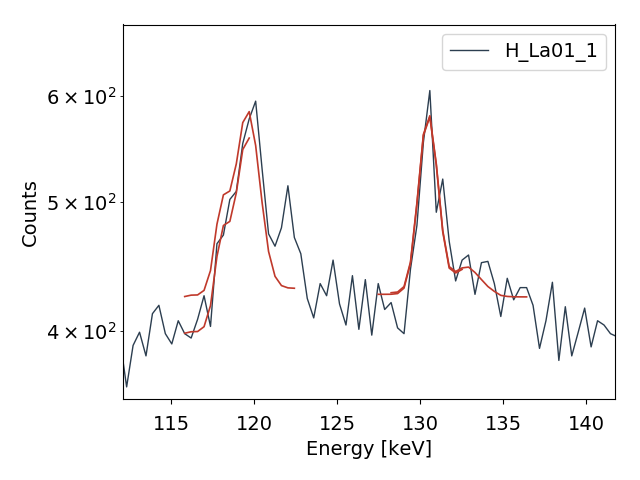
\includegraphics[width=2.5in]{old_fit.png}
\\
\column{2.5in}
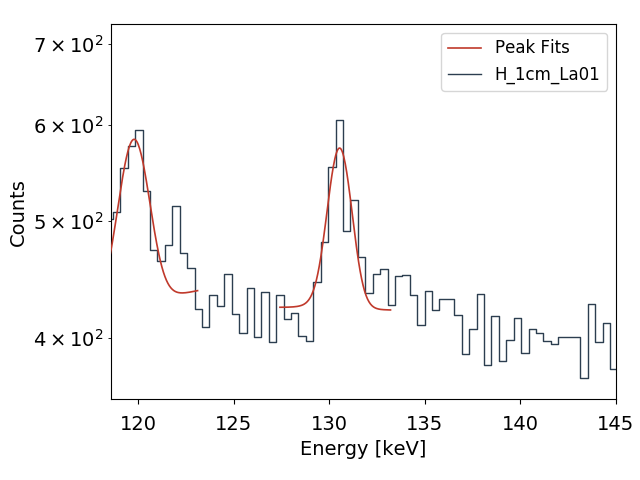
\includegraphics[width=2.5in]{comparison_130.png}
\\
\end{columns}
\end{frame}

\begin{frame}
\frametitle{Other Peak Fits}
\begin{columns}[c]
\column{2.5in}
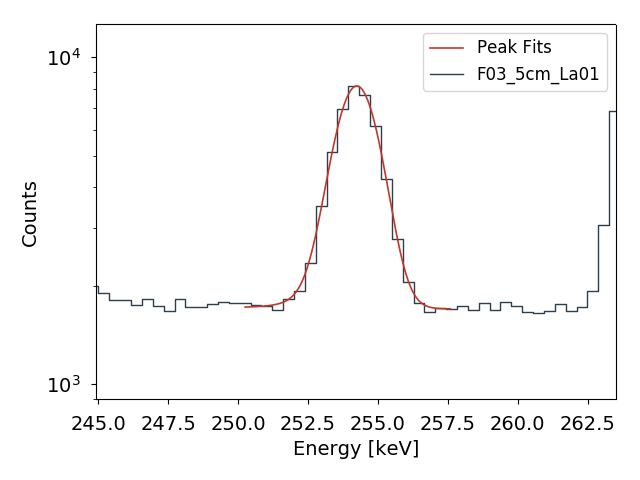
\includegraphics[width=2.5in]{CE137m_fit.png}
\centering
\ \ $^{137m}$Ce: E=254.29 [keV]\\ $I_{\gamma}$=11.1\%\\ $\chi^2_{\nu}$=1.097
\\
\column{2.5in}
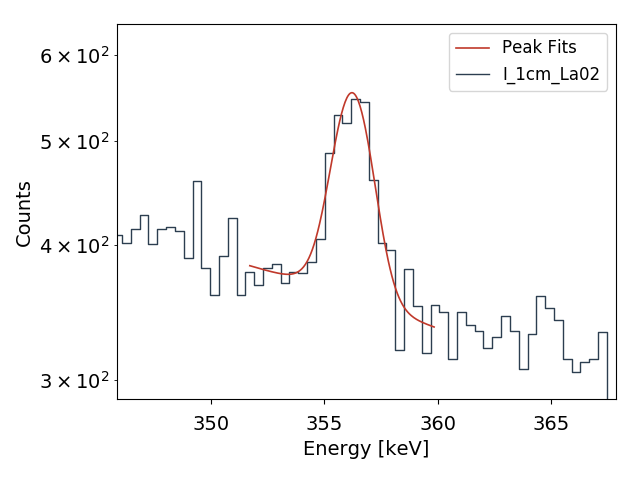
\includegraphics[width=2.5in]{BA133g_fit.png}
\centering
\ \ $^{133g}$Ba: E=356.01 [keV]\\ $I_{\gamma}$=62.05\%\\ $\chi^2_{\nu}$=1.003
\\
\end{columns}
\end{frame}

\begin{frame}
\frametitle{Daughter Nuclide Initial Activities}

$A_D(t_c) = A_{p0}\frac{\lambda_D}{\lambda_D - \lambda_p}(e^{-\lambda_p t_c}-e^{-\lambda_D t_c})+A_{D0}e^{-\lambda_D t_c}$
\\
\centering
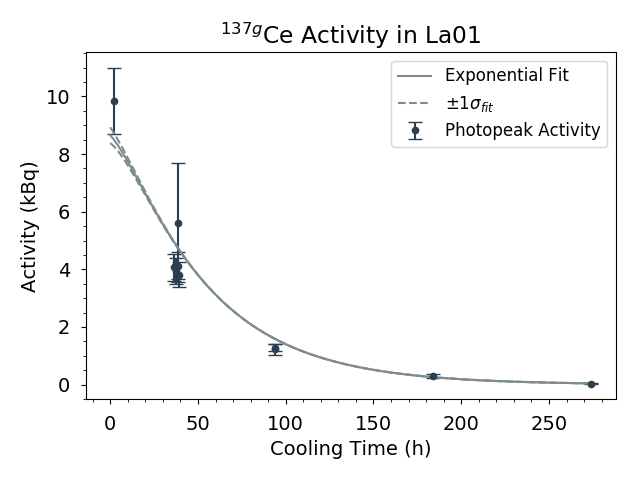
\includegraphics[width=3.5in]{decay_curves/La01_137CEg}
\end{frame}

\begin{frame}
\frametitle{$^{134}$Ce Cross-Section}
\begin{columns}[c]
\column{2.5in}
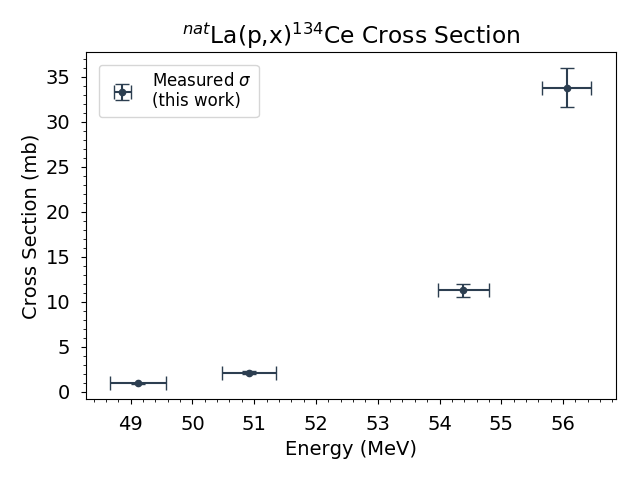
\includegraphics[width=2.5in]{cross_sections/134CE_only}
\\
\column{2.5in}
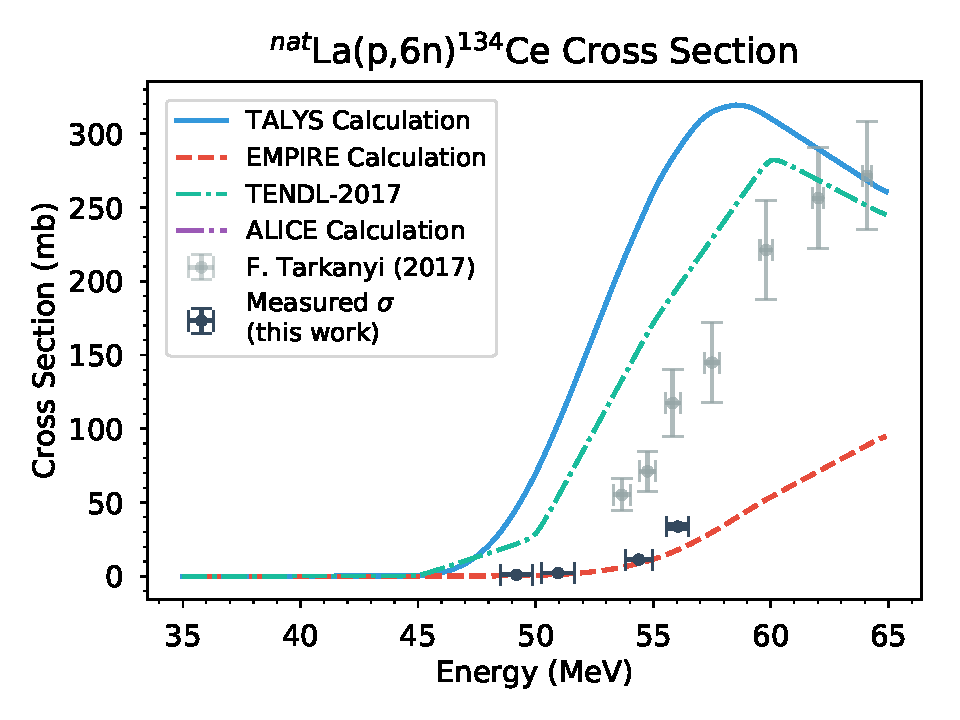
\includegraphics[width=2.5in]{cross_sections/134CE}
\\
\end{columns}
\end{frame}

\begin{frame}
\frametitle{$^{135}$Ce Cross-Section}
\begin{columns}[c]
\column{2.5in}
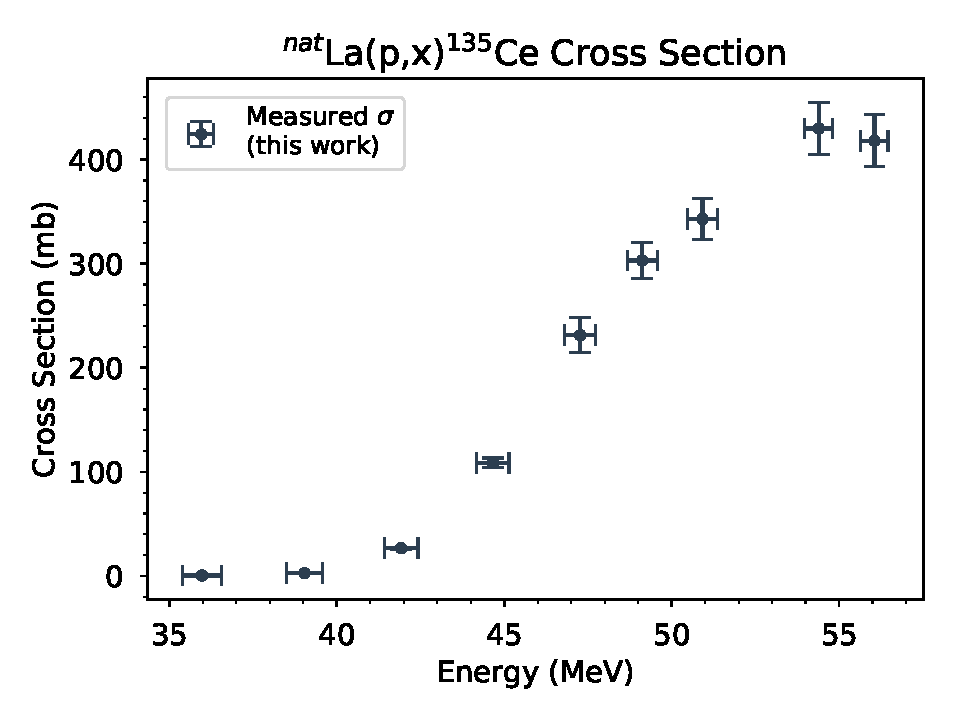
\includegraphics[width=2.5in]{cross_sections/135CE_only}
\\
\column{2.5in}
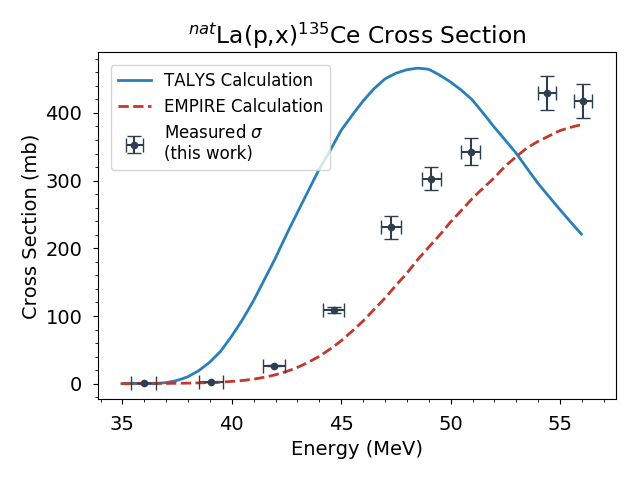
\includegraphics[width=2.5in]{cross_sections/135CE}
\\
\end{columns}
\end{frame}

\begin{frame}
\frametitle{$^{137m}$Ce Cross-Section}
\begin{columns}[c]
\column{2.5in}
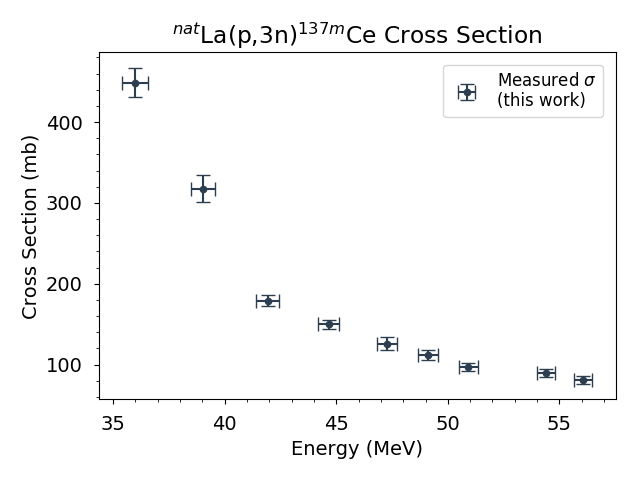
\includegraphics[width=2.5in]{cross_sections/137CEm_only}
\\
\column{2.5in}
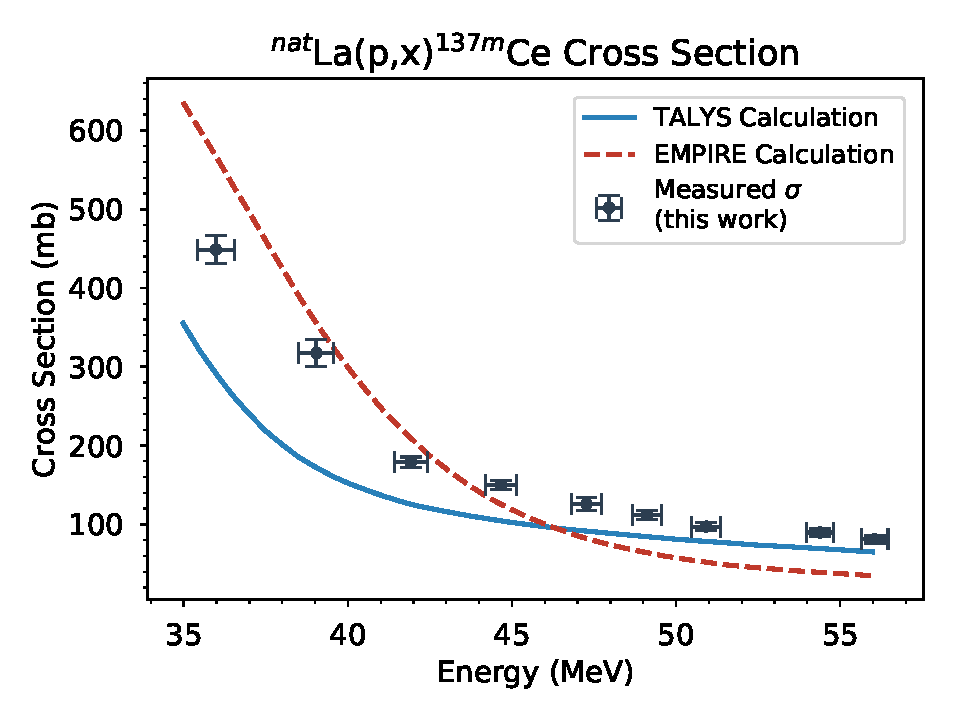
\includegraphics[width=2.5in]{cross_sections/137CEm}
\\
\end{columns}
\end{frame}

\begin{frame}
\frametitle{$^{137g}$Ce Cross-Section}
\begin{columns}[c]
\column{2.5in}
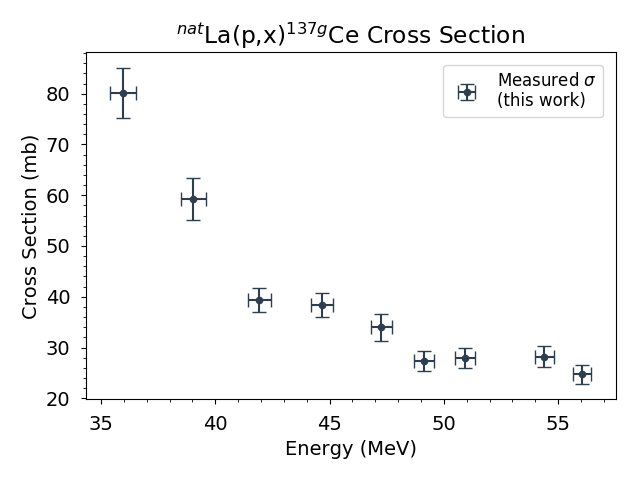
\includegraphics[width=2.5in]{cross_sections/137CEg_only}
\\
\column{2.5in}
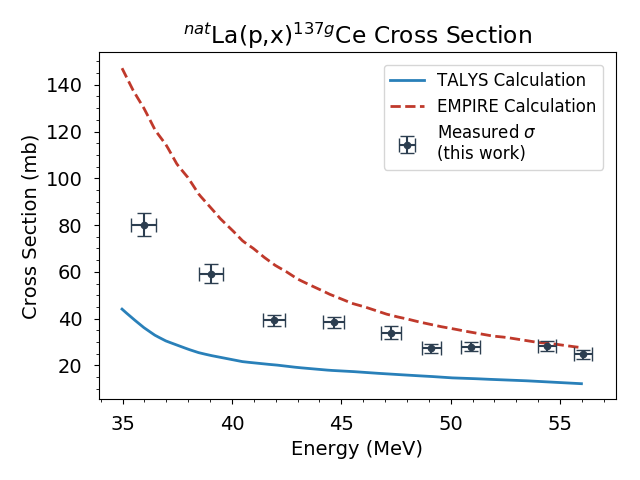
\includegraphics[width=2.5in]{cross_sections/137CEg}
\\
\end{columns}
\end{frame}

\begin{frame}
\frametitle{$^{139}$Ce Cross-Section}
\begin{columns}[c]
\column{2.5in}
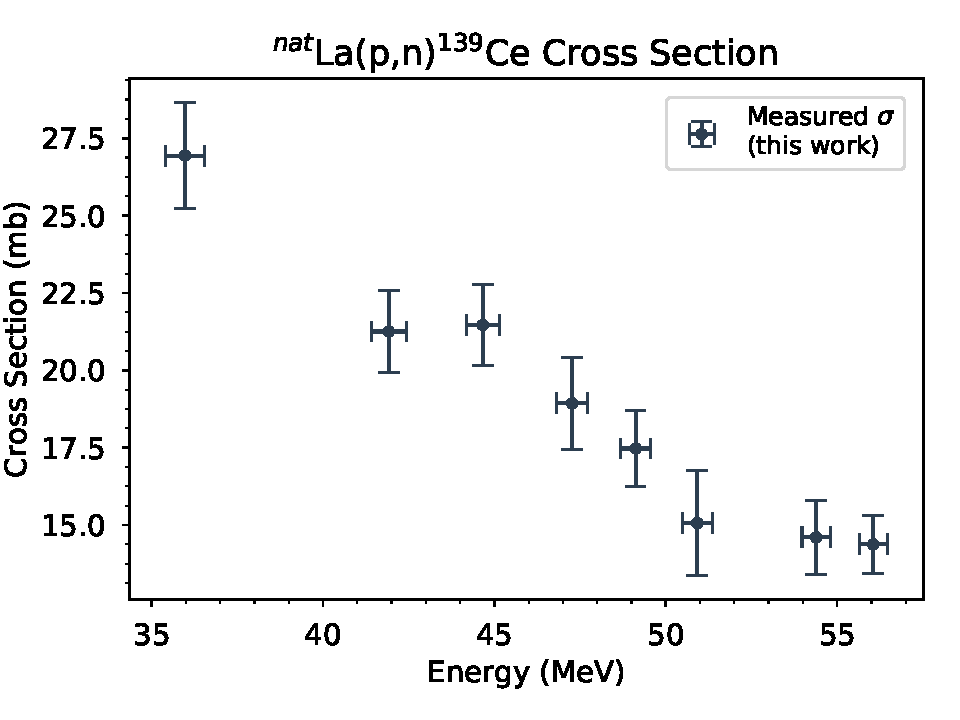
\includegraphics[width=2.5in]{cross_sections/139CE_only}
\\
\column{2.5in}
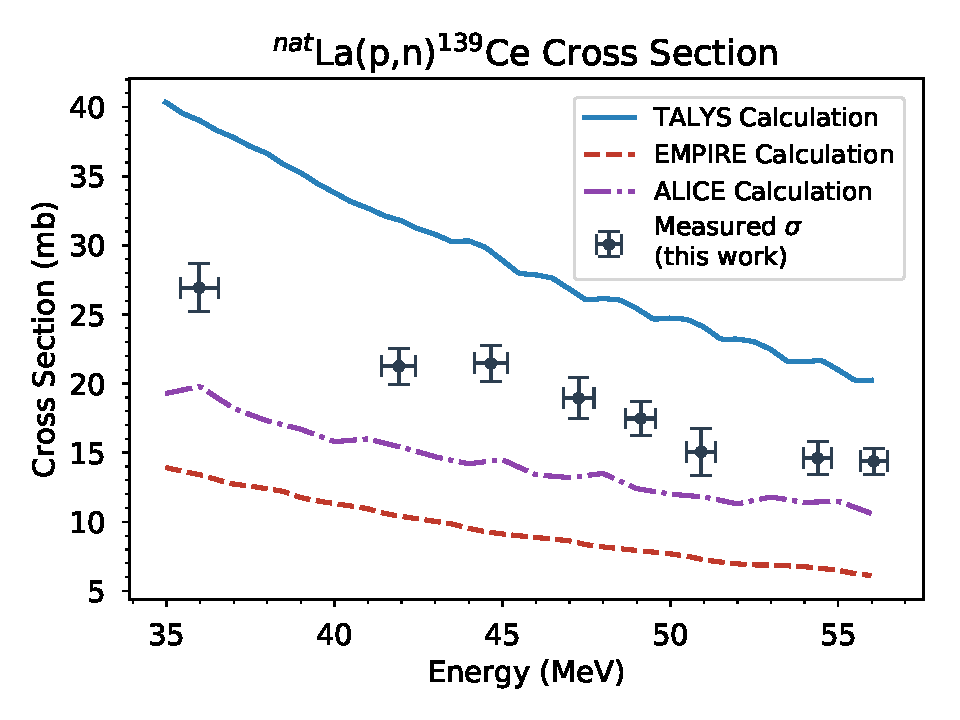
\includegraphics[width=2.5in]{cross_sections/139CE}
\\
\end{columns}
\end{frame}

\begin{frame}
\frametitle{$^{132}$Cs Cross-Section}
\begin{columns}[c]
\column{2.5in}
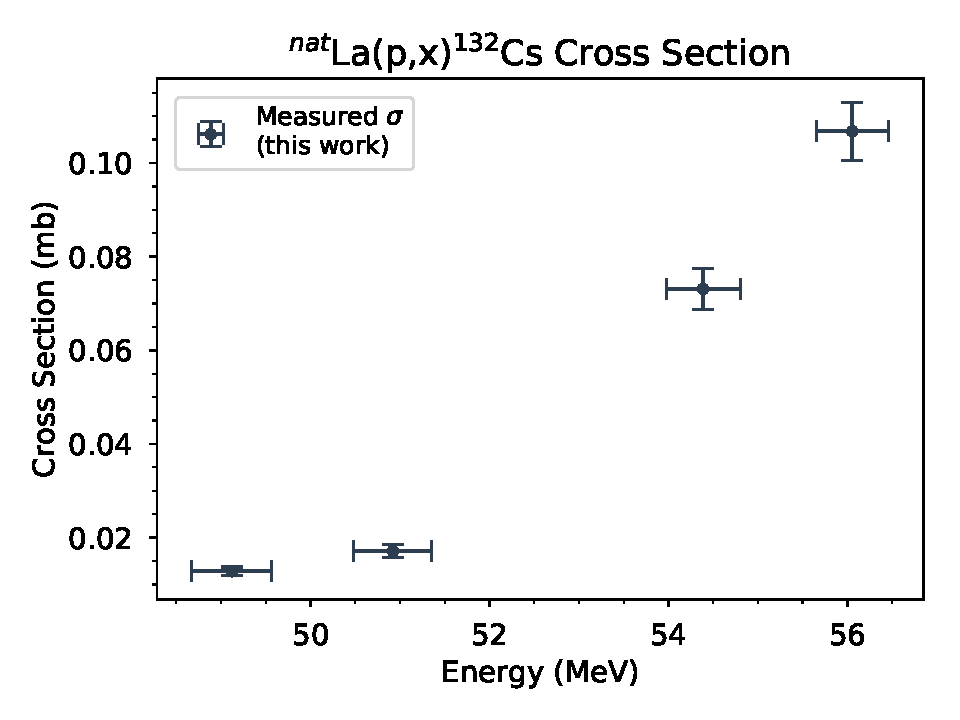
\includegraphics[width=2.5in]{cross_sections/132CS_only}
\\
\column{2.5in}
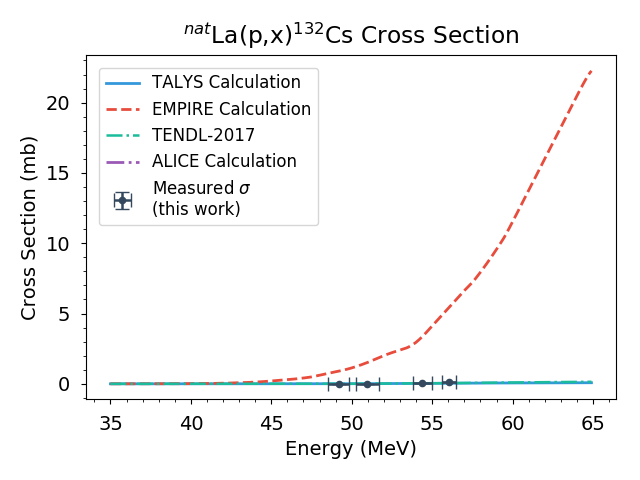
\includegraphics[width=2.5in]{cross_sections/132CS}
\\
\end{columns}
\end{frame}

\begin{frame}
\frametitle{$^{133m}$Ba Cross-Section}
\begin{columns}[c]
\column{2.5in}
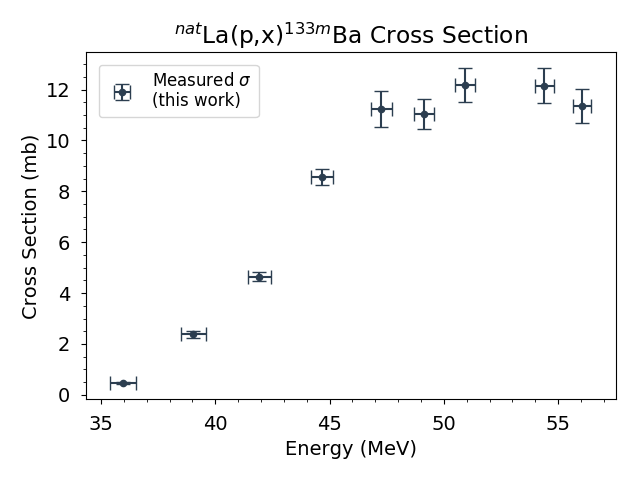
\includegraphics[width=2.5in]{cross_sections/133BAm_only}
\\
\column{2.5in}
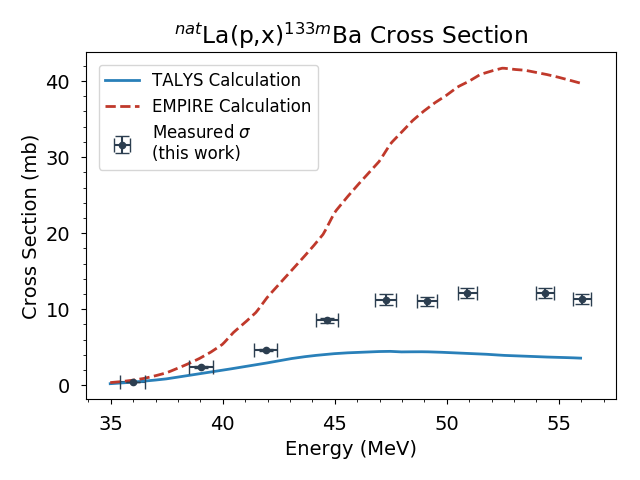
\includegraphics[width=2.5in]{cross_sections/133BAm}
\\
\end{columns}
\end{frame}

\begin{frame}
\frametitle{$^{133g}$Ba Cross-Section}
\begin{columns}[c]
\column{2.5in}
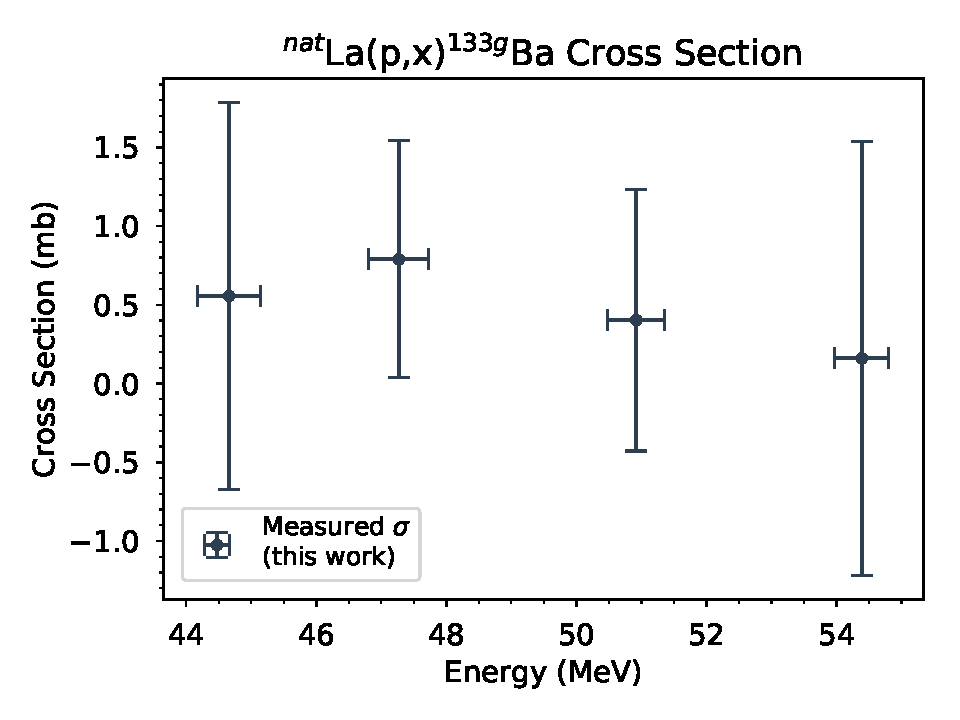
\includegraphics[width=2.5in]{cross_sections/133BAg_only}
\\
\column{2.5in}
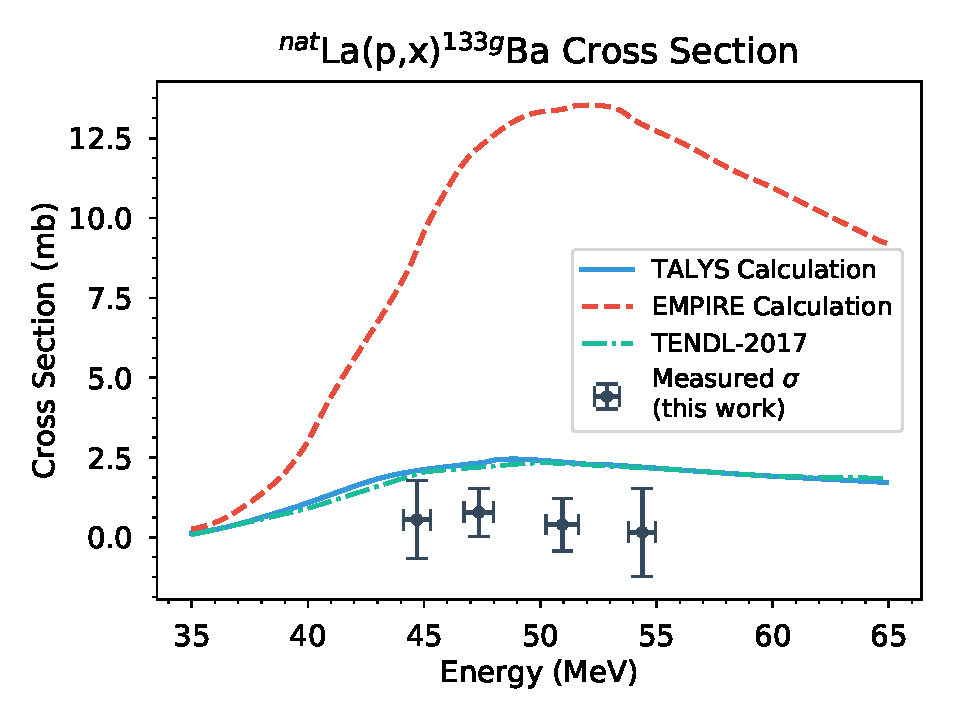
\includegraphics[width=2.5in]{cross_sections/133BAg}
\\
\end{columns}
\end{frame}

\end{document}
